Импорт виртуальной машины

Теперь необходимо скопировать файл на флэшку. Или же можно воспользоваться облочным хранилищем, так как возможно при попытке перенести его на флешку, может возникнуть ошибка: «Файл слишком велик для конечной файловой системы». Она возникает, если передаётся файл размером более четырёх гигабайт на носитель, неспособный с ним работать. Для устранения этой ошибки можно воспользоваться форматированием флешки или разбитием файла с виртуальной машины на несколько частей. Был также опробован способ сжатия виртуальной машины в zip файл, но она оказалась практически без сжимающий составляющих.

Далее на втором компьютере заходим в программу Virtual Box и нажимаем вверху «Файл» и выбираем пункт «Импорт конфигураций».

\begin{figure}[h]
		\centering
		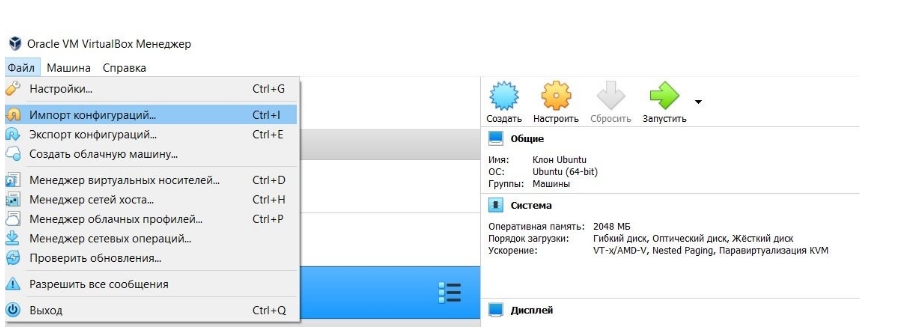
\includegraphics[width=1\linewidth]{VM/14.png}
\caption{Импорт конфигураций.}
\label{ris:image}
\end{figure}

В окне импорта выбираем место размещения файла виртуальной машины, нажимаем «Далее». В следующем окне можно изменить параметры импорта, например, увеличить количество процессоров. Также желательно «Включать (сгенерировать новые) МАС-адреса всех сетевых адаптеров», и нажимаем «Импорт».

Импорт также как и экспорт в зависимости от размера виртуальной машины может занимать несколько минут.

После импорта виртуальная машина появляется в списке и с ней уже можно будет работать.